
\newpage

\begin{center}
	\textbf{\large ГЛАВА 2 \\ КИНЕМАТИЧЕСКАЯ СХЕМА РОБОТА}
\end{center}
\refstepcounter{chapter}


% \section*{}
\addcontentsline{toc}{chapter}{ГЛАВА 2}
\section{Общая схема робота}\label{C2_1}

 %В главе \ref{C1_2} были получены требования к кинематической схеме робота. Необходимо разработать прототип ноги, который представляет из себя двухзвенный механизм с двумя двигателями. Один двигатель расположен ближе к корпусу робота и отвечает за ориентацию положения первого звена, имитирующее бедро робота. Второй двигатель связывает первое и второе звено, которое в свою очередь имитирует голень робота, а также обладает подобием стопы на конце. Конечная кинематическая схема ноги приведена на рисунке \ref{Areaconfig} 
В разделе \ref{C1_2} были определены требования к кинематической конфигурации робота. В целях создания прототипа ноги предложена двухзвенная механическая система, оснащенная двумя двигателями. Первый двигатель расположен ближе к корпусу робота и обеспечивает ориентацию положения первого звена - имитации бедра робота. Второй двигатель связывает первое и второе звено, которое, в свою очередь, имитирует голень робота и завершается элементом, аналогичным стопе. Результирующая кинематическая схема ноги представлена на рисунке \ref{kinematic2D}.

\begin{figure}[ht]
	\begin{center}
		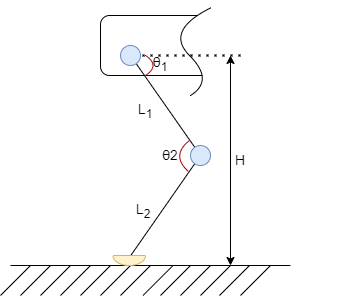
\includegraphics[width=0.5\textwidth]{kinematic2D}
		\caption{Кинематическая схема ноги робота}
		\label{kinematic2D}
	\end{center}
\end{figure}

%Таким образом робот имеет четыре одинаковые ноги. Они прикреплены к туловищу таким образом, что шарнирные соединения передних и задних ног обращены друг от друга, как показано на рисунке 2.2. Каждая нога имеет две степени свободы, одна которых лежит на плечевой части (тазобедренный сустав) и одна на коленном суставе. 
Таким образом, робот имеет четыре одинаковые ноги, каждая из которых имеет две степени свободы. Шарниры передних и задних ног направлены в противоположные стороны и закреплены на туловище, как показано на рисунке \ref{full}. Степени свободы распределены между плечевой частью (тазобедренный сустав) и коленным суставом.

\begin{figure}[h!]
	\begin{center}
		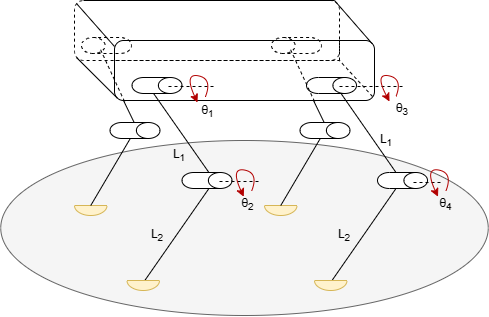
\includegraphics[width=0.8\textwidth]{full}
		\caption{Полная кинематическая схема робота}
		\label{full}
	\end{center}
\end{figure}

\section{Построение рабочей области ноги робота}\label{C2_2}
Для того, чтобы решить обратную задачу кинематики, необходимо определять положения углов с течением времени для совершения шага по некоторой траектории, следовательно, необходимо понимать рабочую область исследуемого объекта, в данном случае ноги. Общие характеристики ноги сведены в таблице \ref{tablParam}


\begin{table}[h]
	\begin{center}
		\caption{Характеристики ног робота}
		\label{tablParam}
		\begin{tabular}{| l | l |}
			\hline
			Общий вес   &    0.2 кг \\ \hline
			Длина первого звена & 100 мм\\ \hline
			Длина второго звена & 100 мм \\ \hline
			Диапазон поворота двигателя (бедро) & $\pm$ 180$^{\circ}$ \\ \hline
			Диапазон поворота двигателя (колено) & $\pm$ 180$^{\circ}$ \\ \hline
		\end{tabular}
	\end{center}
\end{table}

Чтобы описать рабочую область, составим кинематическую схему, представленную на рисунке \ref{Areaconfig} и решим задачу о положении стопы ноги. Точку O будем считать зафиксированной на корпусе. 

Тогда получим уравнения для положения точки B относительно корпуса робота:
\begin{equation}
\begin{array}{l}
	X_{b} = l_{1}\cos{\theta_1}+l_{2}\cos({\theta_1+\theta_2}),
	\\
	Y_{b} = l_{1}\sin{\theta_1}+l_{2}\sin({\theta_1+\theta_2}).
\end{array}
\end{equation}

\begin{figure}[h]
	\begin{center}
		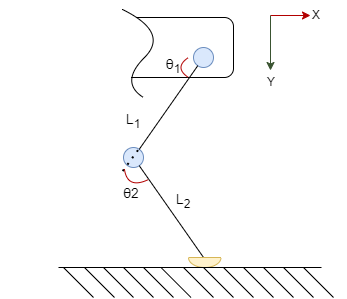
\includegraphics[width=0.5\textwidth]{Areaconfig}
		\caption{Кинематическая схема для определения рабочей области ноги}
		\label{Areaconfig}
	\end{center}
\end{figure}

Используя данные уравнения, которые описывают положение т.B относительно корпуса, а также используя информацию об ограничениях на углы поворота двигателя из таблицы \ref{tablParam}, определим рабочую область ноги (рисунок \ref{workArea}). Алгоритм получения описан в математическом пакете Wolfram Mathematica (Приложение 1). %FIX приложение
\newpage
\begin{figure}[h!]
	\begin{center}
		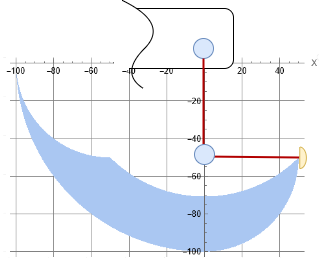
\includegraphics[width=0.8\textwidth]{workArea}
		\caption{Рабочая область ноги робота относительно корпуса}
		\label{workArea}
	\end{center}
\end{figure}

